 % -*- coding: utf-8 -*-
% !TEX program = xelatex

\documentclass[9pt]{beamer}

\usetheme[style=beta]{epyt} % alpha, beta, delta, gamma, zeta
% \usetheme{Warsaw}
\usepackage[UTF8,noindent]{ctex}
\def\blue{\textcolor{blue}}
\def\red{\textcolor{red}}
\def\purple{\textcolor{purple}}
\def\ds{\displaystyle}
\def\cd{\cdots}
\def\dd{\ddots}
\def\vd{\vdots}
\def\id{\iddots}
\def\ft{\frametitle}
\def\diag{\mathrm{diag}}

\def\A{\boldsymbol{A}}
\def\B{\boldsymbol{B}}
\def\C{\boldsymbol{C}}
\def\D{\boldsymbol{D}}
\def\E{\boldsymbol{E}}
\def\F{\boldsymbol{F}}
\def\T{\boldsymbol{T}}
\def\U{\boldsymbol{U}}
\def\X{\boldsymbol{X}}
\def\Y{\boldsymbol{Y}}
\def\Z{\boldsymbol{Z}}
\def\QQ{\boldsymbol{Q}}

\def\R{\mathbb R}
\def\rank{\mathrm{R}}
\def\det{\mathrm{det}}
\def\nn{{\boldsymbol{n}}}
\def\xx{{\boldsymbol{x}}}
\def\yy{{\boldsymbol{y}}}
\def\aa{{\boldsymbol{a}}}
\def\bb{{\boldsymbol{b}}}
\def\ee{{\boldsymbol{e}}}
\def\ii{{\boldsymbol{i}}}
\def\jj{{\boldsymbol{j}}}
\def\kk{{\boldsymbol{k}}}
\def\uu{{\boldsymbol{u}}}
\def\vv{{\boldsymbol{v}}}

\def\tf{\ttfamily}
\def\zero{\boldsymbol{0}}
\def\II{\boldsymbol{I}}
\def\PP{\boldsymbol{P}}
\def\XX{\boldsymbol{X}}
\def\Lambdabd{\boldsymbol{\Lambda}}
\def\alphabd{\boldsymbol{\alpha}}
\def\betabd{\boldsymbol{\beta}}
\def\gammabd{\boldsymbol{\gamma}}
\def\xibd{\boldsymbol{\xi}}
\def\etabd{\boldsymbol{\eta}}
\def\epsilonbd{\boldsymbol{\epsilon}}
\usepackage{multicol}
%\usepackage{fontspec}
\usepackage[most]{tcolorbox}
\newcounter{testexample}
\usepackage{xparse}
\usepackage{lipsum}
\usepackage[UTF8,noindent]{ctex}
\usepackage{extarrows}
%\usepackage{courier}
\usepackage{animate}
\usepackage{dcolumn}
\usepackage{pgf}
\usepackage{tikz}
\usetikzlibrary{calc}
\usetikzlibrary{arrows,snakes,backgrounds,shapes,patterns}
\usetikzlibrary{matrix,fit,positioning,decorations.pathmorphing}
\usepackage{listings}
\lstset{
        language=python,
        keywordstyle=\color{blue!70},
        frame=single,
        basicstyle=\ttfamily,
        commentstyle=\color{red},
        breakindent=0pt,
        rulesepcolor=\color{red!20!green!20!blue!20},
        rulecolor=\color{black},
        tabsize=4,
        numbersep=5pt,
        breaklines=true,
        %% backgroundcolor=\color{red!10},
        showstringspaces=false,
        showspaces=false,
        showtabs=false,
        extendedchars=false,
        escapeinside=``,
        frame=single,
}
\def\exampletext{例} % If English
\NewDocumentEnvironment{testexample}{ O{} }
{
\colorlet{colexam}{red!55!black} % Global example color
\newtcolorbox[use counter=testexample]{testexamplebox}{%
    % Example Frame Start
    empty,% Empty previously set parameters
    title={\exampletext: #1},% use \thetcbcounter to access the testexample counter text
    % Attaching a box requires an overlay
    attach boxed title to top left,
       % Ensures proper line breaking in longer titles
       minipage boxed title,
    % (boxed title style requires an overlay)
    boxed title style={empty,size=minimal,toprule=0pt,top=4pt,left=3mm,overlay={}},
    coltitle=colexam,fonttitle=\bfseries,
    before=\par\medskip\noindent,parbox=false,boxsep=0pt,left=3mm,right=0mm,top=2pt,breakable,pad at break=0mm,
       before upper=\csname @totalleftmargin\endcsname0pt, % Use instead of parbox=true. This ensures parskip is inherited by box.
    % Handles box when it exists on one page only
    overlay unbroken={\draw[colexam,line width=.5pt] ([xshift=-0pt]title.north west) -- ([xshift=-0pt]frame.south west); },
    % Handles multipage box: first page
    overlay first={\draw[colexam,line width=.5pt] ([xshift=-0pt]title.north west) -- ([xshift=-0pt]frame.south west); },
    % Handles multipage box: middle page
    overlay middle={\draw[colexam,line width=.5pt] ([xshift=-0pt]frame.north west) -- ([xshift=-0pt]frame.south west); },
    % Handles multipage box: last page
    overlay last={\draw[colexam,line width=.5pt] ([xshift=-0pt]frame.north west) -- ([xshift=-0pt]frame.south west); },%
    }
\begin{testexamplebox}}
{\end{testexamplebox}\endlist}





\begin{document}

\title{数据结构与算法}
\subtitle{引言}
\author{张晓平}
\institute{武汉大学数学与统计学院}


\begin{frame}[plain]\transboxout
  \titlepage
\end{frame}

\section*{目录}
\frame{  
  \frametitle{\secname}
  \begin{multicols}{2}  %两行目录
    \tableofcontents
  \end{multicols}
}
\AtBeginSection[] {  %在每个subsection前面显示一次目录
  \frame{
    \begin{multicols}{2}  %两行目录
      \tableofcontents[current,currentsection]
    \end{multicols}
  }
}

\AtBeginSubsection[] {  %在每个subsection前面显示一次目录
  \frame{
    \begin{multicols}{2}  %两行目录
      \tableofcontents[current,currentsubsection]
    \end{multicols}
  }
}


%\section{目标}
\begin{frame}\ft{\secname}
% \begin{itemize}
% \item 回顾计算机科学的思想, 提高编程和解决问题的能力。
% \item 理解抽象化以及它在解决问题过程中发挥的作用
% \item 理解和实现抽象数据类型的概念
% \item 回顾 Python 编程语言
% \end{itemize}
\end{frame}

% \section{快速开始}

\begin{frame}\ft{\secname}
  \begin{itemize}
  \item 计算技术的变化为计算机科学家提供了越来越多的工具和平台。
  \item 计算机的快速发展,诸如快速处理器、高速网络和大容量存储器,已经让计算机科学家陷入高度复杂螺旋中。
  \end{itemize}

  在所有这些快速演变中,有一些基本原则会保持不变。计算机科学关注用计算机来解决问题。
\end{frame}


\begin{frame}\ft{\secname}
  %或许你花了很多时间学习了解决问题的基础知识,希望自己能把问题弄清楚并提出解决方案。接着你可能还会发现编程有些难。
  问题以及解决方案的复杂性可能会掩盖求解过程中的一些基本思想。
\end{frame}


\begin{frame}\ft{\secname}


简要回顾计算机科学、算法和数据结构所必须适应的框架,研究其原因,以及如何理解它们以有助于更好的解决问题。
\end{frame}


% \section{什么是计算机科学}

\begin{frame}\ft{\secname}
  所谓计算机科学,即
  \begin{itemize}
  \item 研究问题
  \item 解决问题
  \item 生成解决问题的方案
  \end{itemize}
  给定一个问题,目标是开发算法,编写程序,用于解决可能出现的问题。%算法遵循它有限的过程就可以解决问题。
\end{frame}

% \begin{frame}\ft{\secname}
% 计算机科学可以被认为是对算法的研究。但是,我们必须清楚地认识到,一些问题可能没有解决方案。虽然证明这种说法正确性超出了本文的范围,但一些问题不能解决的事实对于那些研究计算机科学的人是很重要的。可以这么说,计算机科学研究有解决方案和没有解决方案的问题。
% \end{frame}

% \begin{frame}\ft{\secname}
% 当描述问题及其解决方案时,会提到计算一词。若存在一个算法解决某个问题,就称该问题是可计算的。计算机科学的另一个定义是:计算机科学是研究那些可计算和不可计算的问题,研究是不是存在一种算法来解决它。请注意这里没有涉及到“计算机”一词,解决方案与机器无关。
% \end{frame}

\begin{frame}\ft{\secname}
计算机科学,因涉及问题解决过程本身,是关于抽象的研究。抽象使我们能从逻辑视角和物理视角来分别看待问题及其解决方案。%基本思想跟我们常见的例子一样。
\end{frame}

\begin{frame}\ft{\secname}
  \begin{figure}
  	\centering
  	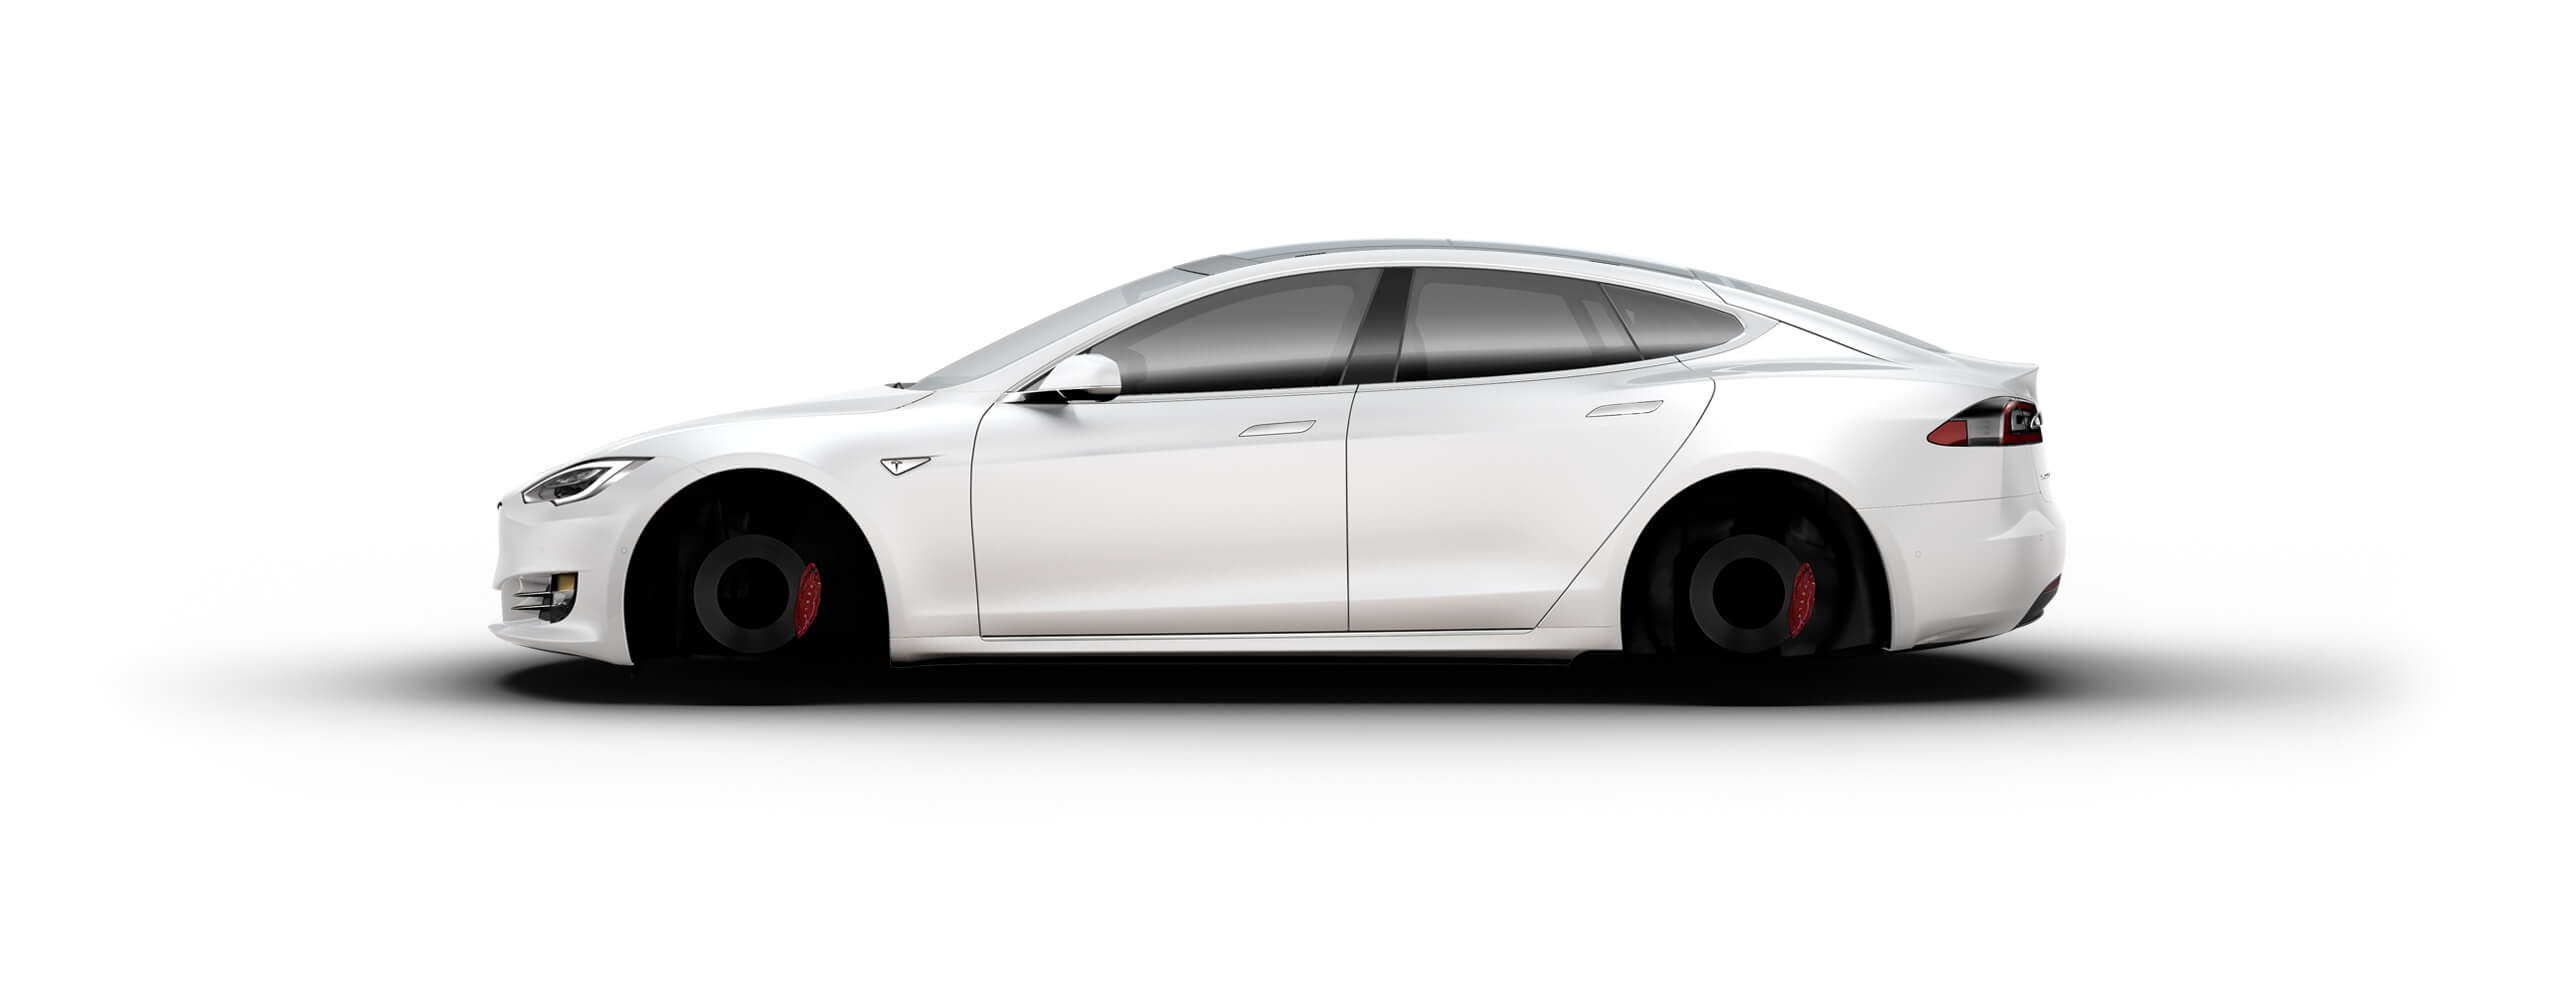
\includegraphics[width=3.5in]{images/car.jpg}
  \end{figure} \pause 
  \begin{itemize}
  \item   作为司机,你会与车有一些互动,如上车、插钥匙、点火、换挡、制动、加速、转向、下车等。你只需要了解车一些基本功能,就可以操纵它。\\
  \item[] 此时,你所看到的是汽车的“逻辑视角”,这些功能通常称为“接口”。 \\[0.1in] \pause 
  
  \item   作为修车师傅,看待汽车的视角就会截然不同。你不仅需要知道如何开车,还必须知道汽车的一些内部细节,比如说发动机如何工作、变速箱如何变速、温度如何控制等等。
  \item[] 这就是“物理视角”,细节发生在“引擎盖下”。
    
  \end{itemize}
\end{frame}

\begin{frame}\ft{\secname}
  \begin{figure}
  	\centering
  	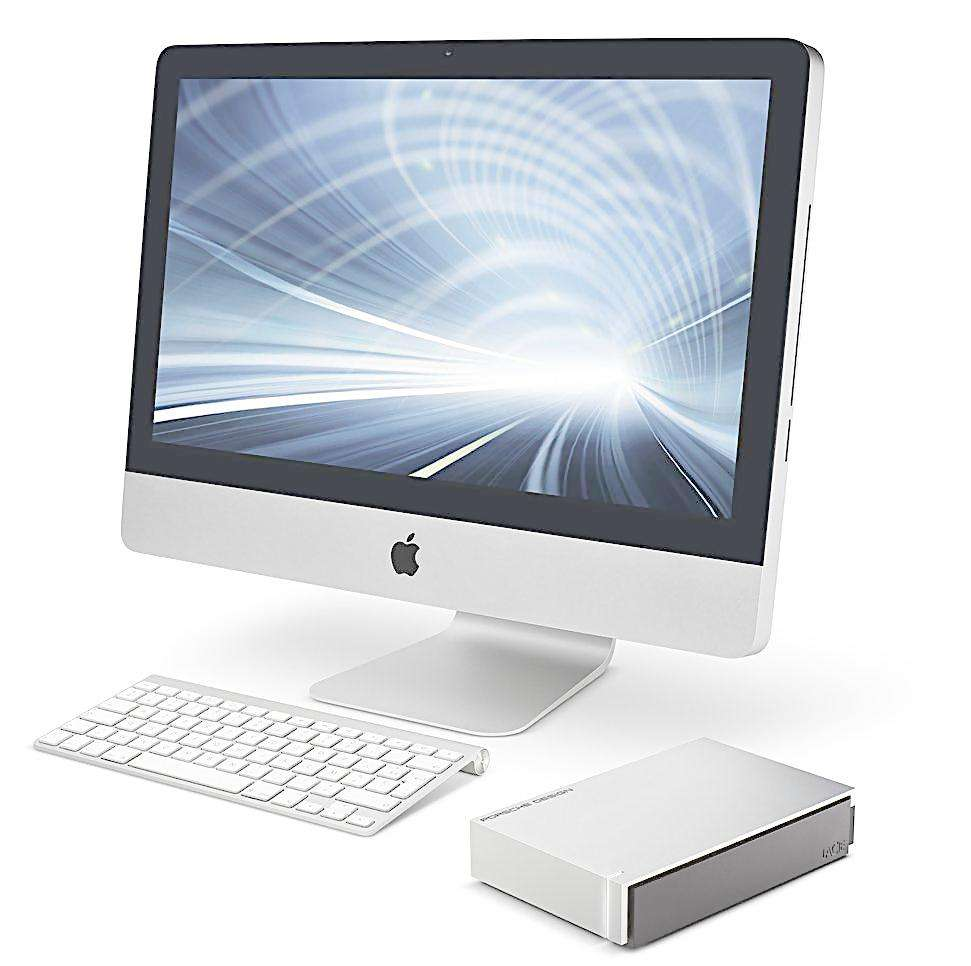
\includegraphics[width=1.5in]{images/computer.jpeg}
  \end{figure} \pause 
  \begin{itemize}
  \item 作为用户,你可以编写文档、收发邮件、上网冲浪、播放音乐、存储图像和玩游戏等,但你并不知道这些APP工作的细节。
  \item[] 此时,你是从逻辑或用户角度看待计算机。 \\[0.1in] \pause 
  \item 作为计算机科学家、程序员、技术支持人员和系统管理员,你看待计算机的角度会截然不同。你必须知道操作系统如何工作、如何配置网络协议、如何编写控制功能的各种脚本。
  \item[] 总之,你必须能够控制底层的细节。

  \end{itemize}

\end{frame}

\begin{frame}[fragile]\ft{\secname}

  作为用户,你不需要知道细节,只需了解接口的工作方式。接口是用户与底层沟通的窗口。

\end{frame}

\begin{frame}[fragile]\ft{\secname}

  看一个抽象的例子---Python 数学模块。一旦导入模块,就可以执行计算
\begin{lstlisting}
  >>> import math
  >>> math.sqrt(16)
  4.0
\end{lstlisting} \pause 

你无需知道计算平方根的细节,只需知道sqrt函数的功能及其使用方式。这就像一个“黑盒子”,其接口可描述为:函数名、参数、返回值,其细节隐藏在内部。
\begin{figure}[htbp]
  \centering
  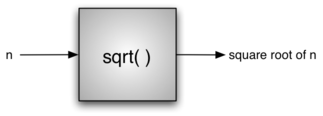
\includegraphics[width=2in]{images/blackbox.png}
\end{figure}

\end{frame}


% \section{什么是编程}

\begin{frame}\ft{\secname}
  编程是将算法转换为程序语言的过程,以便能被计算机所执行。

  \begin{itemize}
  \item 首先要有解决方案,亦即算法;
  \item 然后在选择合适的编程语言实现算法。
  \end{itemize}
  计算机科学不研究编程,但编程却是计算机科学家的重要能力。编程通常是解决方案的表达方式。
\end{frame}

\begin{frame}\ft{\secname}
  \begin{itemize}
  \item 算法描述了依据实际问题所生成的解决方案和产生预期结果所需要的一套步骤。

  \item 编程语言必须提供一种表示方法来表示对应的过程和数据。为此,它提供了\red{控制结构}和\red{数据类型}。
  \end{itemize}
\end{frame}

\begin{frame}\ft{\secname}
\red{控制结构}允许以方便而明确的方式表示算法步骤。至少,算法需要执行顺序处理、决策选择和控制迭代。只要语言提供这些基本语句,它就可以表达算法。
\end{frame}

\begin{frame}\ft{\secname}
  在计算机中,所有数据项都由一串一串的二进制数表示。为了让这些二进制串有意义,就需要有\red{数据类型}。 
  \begin{itemize}
  \item 数据类型为二进制数据提供解释,以便我们能够根据实际问题来思考数据。
    这些底层的内置数据类型(有时称为原始数据类型)为算法开发提供了基础。 \pause 
  \item[] 
    例如,大多数编程语言提供整数类型。内存中的二进制数据可解释为整数,并且给予一个与整数(如 23, 654 和 -19)相关联的含义。 \pause \\[0.1in]
  \item   此外,数据类型还提供数据项所参与操作的描述。对于整数,提供诸如加法、减法和乘法的操作。%我们期望数值类型的数据可以参与这些算术运算。
  \end{itemize}
% \end{frame}

% \begin{frame}\ft{\secname}
  
\end{frame}

\begin{frame}\ft{\secname}
  然而,通常我们遇到的困难是问题及其解决方案非常复杂。由语言提供的简单的结构和数据类型,虽然可以表示复杂的解决方案,但在实际中却不好用。
  我们需要一些方法控制这种复杂性,以助于形成更好的解决方案。
\end{frame}
% \section{为什么要学习数据结构和抽象数据类型}
\begin{frame}\ft{\secname}
  为管理问题的复杂性及解决过程,计算机科学家使用抽象使他们能够专注于 “大局” 而不会迷失在细节中。\vskip.1in

  通过对问题进行建模,我们能够更好和更有效地解决问题。\vskip.1in


  这些模型允许我们以更加一致的方式来描述我们的算法。
\end{frame}

\begin{frame}\ft{\secname}
  \begin{itemize}
  \item \blue{过程抽象}:隐藏特定函数的细节,以允许用户或客户端在高层查看它。\\[0.1in] \pause 
  \item \blue{数据抽象,即抽象数据类型(ADT)}:对数据和允许操作的逻辑描述,不用考虑如何实现它们。
  \item[] 这意味着我们只关心数据表示什么,而不关心它最终将如何构造。通过提供这种级别的抽象,我们围绕数据创建一个封装。通过封装实现细节,我们将它们从用户的视图中隐藏。这称为信息隐藏。
  \end{itemize}

\end{frame}

\begin{frame}\ft{\secname}

\begin{figure}[htbp]
  \centering
  
\includegraphics[width=4in]{images/ds_adt.png}
  \caption{展示了ADT是什么以及如何操作。用户与接口交互,使用抽象数据类型指定的操作。抽象数据类型是用户与之交互的 shell。实现隐藏在更深的底层。用户不关心实现的细节。}
\end{figure}
\end{frame}

\begin{frame}\ft{\secname}
  ADT的实现要求我们使用一些程序构建和原始数据类型的集合来提供数据的物理视图。

  “逻辑”与“物理”两个视角的分离,允许我们将问题定义复杂的数据模型,而不给出关于模型如何实际构建的细节。
  这提供了独立于实现的数据视图。


  由于通常有许多不同的方法来实现抽象数据类型,所以这种实现独立性允许程序员在不改变数据的用户与其交互的方式的情况下切换实现的细节。

  用户可以继续专注于解决问题的过程。
\end{frame}


% \section{为什么要学习算法}
\begin{frame}\ft{\secname}
计算机科学家经常通过经验学习。我们通过看别人解决问题和自己解决问题来学习。接触不同的问题解决技术,看不同的算法设计有助于我们面对下一个具有挑战性的问题。通过思考许多不同的算法,我们可以开始开发模式识别,以便下一次出现类似的问题时,我们能够更好地解决它。
\end{frame}

\begin{frame}\ft{\secname}
  算法通常彼此完全不同。例如,对于 sqrt,完全可能存在很多不同的方式来实现其细节。

  自然地,我们建议使用一个更高效,或者一个只是工作更快或使用更少的内存的算法。

  %当我们研究算法时,我们可以学习分析技术,允许我们仅仅根据自己的特征而不是用于实现它们的程序或计算机的特征来比较和对比解决方案。
\end{frame}

% \begin{frame}\ft{\secname}
% 在最坏的情况下,我们可能有一个难以处理的问题,这意味着没有算法可以在实际的时间量内解决问题。重要的是能够区分具有解决方案的那些问题,不具有解决方案的那些问题,以及存在解决方案但需要太多时间或其他资源来合理工作的那些问题。
% \end{frame}

\begin{frame}\ft{\secname}
  % 经常需要权衡,我们需要做决定。
  作为计算机科学家,除了需要具备解决问题的能力,还需要掌握解决方案的评估技术。

  
  通常有很多方法来解决问题,所以当我们找到一个解决方案时,需要一遍又一遍地进行比较,然后决定它是否是一个好的方案。

\end{frame}


\section{Numpy}
\begin{frame}
%Numpy is the core library for scientific computing in Python. It provides a high-performance multidimensional array object, and tools for working with these arrays. If you are already familiar with MATLAB, you might find this tutorial useful to get started with Numpy.

Numpy 是 Python 中用于科学计算的核心库。它提供一个高性能的多维数据对象,以及相关工具。 
\end{frame}

\subsection{数组}
\begin{frame}


%A numpy array is a grid of values, all of the same type, and is indexed by a tuple of nonnegative integers. The number of dimensions is the rank of the array; the shape of an array is a tuple of integers giving the size of the array along each dimension.
%
%We can initialize numpy arrays from nested Python lists, and access elements using square brackets:

一个numpy数组是一个由不同数值组成的网格。网格中的数据都是同一种数据类型,可以通过非负整型数的元组来访问。维度的数量被称为数组的阶,数组的大小是一个由整型数构成的元组,可以描述数组不同维度上的大小。
\end{frame}

\begin{frame}
我们可以从列表创建数组,然后利用方括号访问其中的元素:


\lstinputlisting[]{code/np_array1.py}
\end{frame}

\begin{frame}

%Numpy also provides many functions to create arrays:

Numpy还提供了很多其他创建数组的方法:
\lstinputlisting[]{code/np_array2.py}
\end{frame}

\subsection{访问数组}

\begin{frame}

%Numpy offers several ways to index into arrays.
%
%Slicing: Similar to Python lists, numpy arrays can be sliced. Since arrays may be multidimensional, you must specify a slice for each dimension of the array:

Numpy提供了多种访问数组的方法。
\end{frame}

\begin{frame}

切片:和Python列表类似,numpy数组也可以使用切片语法。因为数组可以是多维的,所以你必须为每个维度指定好切片。


\lstinputlisting[]{code/np_array_slice.py}

\end{frame}

\begin{frame}

%You can also mix integer indexing with slice indexing. However, doing so will yield an array of lower rank than the original array. Note that this is quite different from the way that MATLAB handles array slicing:

你可以同时使用整型和切片语法来访问数组。但是,这样做会产生一个比原数组低阶的新数组。需要注意的是,这里和MATLAB中的情况是不同的:

\lstinputlisting[]{code/np_array_shape.py}


\end{frame}

\begin{frame}

%Integer array indexing: When you index into numpy arrays using slicing, the resulting array view will always be a subarray of the original array. In contrast, integer array indexing allows you to construct arbitrary arrays using the data from another array. Here is an example:

整型数组访问:当我们使用切片语法访问数组时,得到的总是原数组的一个子集。整型数组访问允许我们利用其它数组的数据构建一个新的数组:


\lstinputlisting[]{code/np_integer_array_index.py}
\end{frame}

\begin{frame}

%One useful trick with integer array indexing is selecting or mutating one element from each row of a matrix:

整型数组访问语法还有个有用的技巧,可以用来选择或者更改矩阵中每行中的一个元素:
\lstinputlisting[]{code/np_integer_array_index1.py}

\end{frame}

\begin{frame}

%Boolean array indexing: Boolean array indexing lets you pick out arbitrary elements of an array. Frequently this type of indexing is used to select the elements of an array that satisfy some condition. Here is an example:

布尔型数组访问:布尔型数组访问可以让你选择数组中任意元素。通常,这种访问方式用于选取数组中满足某些条件的元素,举例如下:

\lstinputlisting[]{code/np_boolean_array_index.py}
\end{frame}

\begin{frame}

为了教程的简洁,有很多数组访问的细节我们没有详细说明,可以查看\href{http://docs.scipy.org/doc/numpy/reference/arrays.indexing.html}{文档}。
\end{frame}

\subsection{数据类型}

\begin{frame}


%Every numpy array is a grid of elements of the same type. Numpy provides a large set of numeric datatypes that you can use to construct arrays. Numpy tries to guess a datatype when you create an array, but functions that construct arrays usually also include an optional argument to explicitly specify the datatype. Here is an example:

每个Numpy数组都是数据类型相同的元素组成的网格。Numpy提供了很多的数据类型用于创建数组。当你创建数组的时候,Numpy会尝试猜测数组的数据类型,你也可以通过参数直接指定数据类型,例子如下:
\lstinputlisting[]{code/np_datatype.py}

\end{frame}
\subsection{Array math}

\begin{frame}[allowframebreaks]

%Basic mathematical functions operate elementwise on arrays, and are available both as operator overloads and as functions in the numpy module:
基本数学函数会对数组进行逐元计算,既可以利用操作符重载,也可以使用函数方式:


\lstinputlisting[]{code/np_array_math.py}
\end{frame}


\begin{frame}
%Note that unlike MATLAB, * is elementwise multiplication, not matrix multiplication. We instead use the dot function to compute inner products of vectors, to multiply a vector by a matrix, and to multiply matrices. dot is available both as a function in the numpy module and as an instance method of array objects:

不同于MATLAB,* 是逐元乘法,而不是矩阵乘法。在 numpy 中,使用 dot 函数计算向量的的内积、矩阵向量乘法、矩阵乘法。%dot 可作为 numpy 模块的一个函数,也可以作为数组对象的一个实例方法:
\lstinputlisting[]{code/np_dot.py}

\end{frame}


\begin{frame}

%Numpy provides many useful functions for performing computations on arrays; one of the most useful is sum:

  Numpy 提供很多计算数组的函数。


  其中最常用的一个是 sum :
\lstinputlisting[]{code/np_sum.py}
\end{frame}


\begin{frame}[allowframebreaks]

其他一些数学函数:
\lstinputlisting[]{code/np_math.py}

想要了解更多数学函数,可以查看\href{http://docs.scipy.org/doc/numpy/reference/routines.math.html}{文档}。

\end{frame}

\begin{frame}


%Apart from computing mathematical functions using arrays, we frequently need to reshape or otherwise manipulate data in arrays. The simplest example of this type of operation is transposing a matrix; to transpose a matrix, simply use the T attribute of an array object:

除了计算,我们还常常改变数组或者操作其中的元素。其中将矩阵转置是常用的一个,在Numpy中,使用T来转置矩阵:
\lstinputlisting[]{code/np_transpose.py}

\end{frame}
\subsection{广播机制(Broadcasting)}

\begin{frame}


%Broadcasting is a powerful mechanism that allows numpy to work with arrays of different shapes when performing arithmetic operations. Frequently we have a smaller array and a larger array, and we want to use the smaller array multiple times to perform some operation on the larger array.

%For example, suppose that we want to add a constant vector to each row of a matrix. We could do it like this:

%广播是一种强有力的机制,它允许numpy在实现算术操作时去处理不同不同shape的数组。假设有一个小数组和一个大数组,我们想多次使用小数组去对大数组做某些操作。例如,假设我们想对矩阵的每一行加上一个常向量,可以这么做:

  广播是一种强有力的机制,它允许 numpy 让不同大小的矩阵在一起进行数学计算。我们常常会有一个小的矩阵和一个大的矩阵,然后我们会需要用小的矩阵对大的矩阵做一些计算。

  举个例子,如果我们想要把一个向量加到矩阵的每一行,我们可以这样做:
  \lstinputlisting[]{code/np_broadcast.py}
\end{frame}

\begin{frame}
%This works; however when the matrix x is very large, computing an explicit loop in Python could be slow. Note that adding the vector v to each row of the matrix x is equivalent to forming a matrix vv by stacking multiple copies of v vertically, then performing elementwise summation of x and vv. We could implement this approach like this:
这样是行得通的,但是当x矩阵非常大,利用循环来计算就会变得很慢很慢。我们可以换一种思路:

% %可以这么做;然而当矩阵 x 很大时,在 Python 中计算一个显示的循环会很慢。注意对矩阵 x 的每一行加上向量 v 等价于通过按垂直方向复制 v 若干次而叠加成一个矩阵 vv,然后对 x 和 vv 进行逐元加法。我们可以这样实现这一过程: 


\lstinputlisting[]{code/np_broadcast1.py}

\end{frame}

\begin{frame}

%Numpy broadcasting allows us to perform this computation without actually creating multiple copies of v. Consider this version, using broadcasting:

%Numpy 广播机制允许我们不需要真正地创建v的多重拷贝来执行这一计算。使用广播机制,我们可以这么做:

Numpy广播机制可以让我们不用创建vv,就能直接运算,看看下面例子:


\lstinputlisting[]{code/np_broadcast2.py}


% %The line y = x + v works even though x has shape (4, 3) and v has shape (3,) due to broadcasting; this line works as if v actually had shape (4, 3), where each row was a copy of v, and the sum was performed elementwise.

\pause 
由于广播机制,即使 x 有shape (4, 3), v 有shape (3,),\lstinline|y = x + v| 仍可工作; 这就如同 v 有shape (4, 3),其中每一行为v的拷贝,求和按逐元进行。

\end{frame}

\begin{frame}


% Broadcasting two arrays together follows these rules:
% \begin{enumerate}
% \item If the arrays do not have the same rank, prepend the shape of the lower rank array with 1s until both shapes have the same length.
% \item The two arrays are said to be compatible in a dimension if they have the same size in the dimension, or if one of the arrays has size 1 in that dimension.
% \item The arrays can be broadcast together if they are compatible in all dimensions.
% \item After broadcasting, each array behaves as if it had shape equal to the elementwise maximum of shapes of the two input arrays.
% \item In any dimension where one array had size 1 and the other array had size greater than 1, the first array behaves as if it were copied along that dimension
% \item If this explanation does not make sense, try reading the explanation from the documentation or this explanation.
% \end{enumerate}

广播两个数组遵循以下原则:
\begin{enumerate}
\item 如果数组的秩不同,使用1来将秩较小的数组进行扩展,直到两个数组的尺寸的长度都一样。
\item 如果两个数组在某个维度上的长度是一样的,或者其中一个数组在该维度上长度为1,那么我们就说这两个数组在该维度上是相容的。
\item 如果两个数组在所有维度上都是相容的,他们就能使用广播。
\item 如果两个输入数组的尺寸不同,那么注意其中较大的那个尺寸。因为广播之后,两个数组的尺寸将和那个较大的尺寸一样。
\item 在任何一个维度上,如果一个数组的长度为1,另一个数组长度大于1,那么在该维度上,就好像是对第一个数组进行了复制。
\end{enumerate}

% 如果上述解释看不明白,可以读一读\href{http://docs.scipy.org/doc/numpy/user/basics.broadcasting.html}{文档}和这个\href{http://wiki.scipy.org/EricsBroadcastingDoc}{解释}。
% %Functions that support broadcasting are known as universal functions. You can find the list of all universal functions in the documentation.
% %
% %Here are some applications of broadcasting:
\end{frame}

\begin{frame}[allowframebreaks]

%支持广播机制的函数是全局函数。%哪些是全局函数可以在\href{http://docs.scipy.org/doc/numpy/reference/ufuncs.html#available-ufuncs}{文档}中查找。

下面是一些广播机制的使用:

\lstinputlisting[]{code/np_broadcast3.py}

%Broadcasting typically makes your code more concise and faster, so you should strive to use it where possible.

广播机制能够让你的代码更简洁更迅速,能够用的时候请尽量使用!
\end{frame}
\section{SciPy}
\begin{frame}
%Numpy provides a high-performance multidimensional array and basic tools to compute with and manipulate these arrays. SciPy builds on this, and provides a large number of functions that operate on numpy arrays and are useful for different types of scientific and engineering applications.

Numpy提供了高性能的多维数组,以及计算和操作数组的基本工具。 Scipy基于 Numpy,提供了大量的处理numpy数组的函数,这些函数对于不同类型的科学和工程计算非常有用。

熟悉SciPy的最好方法就是阅读\href{http://docs.scipy.org/doc/scipy/reference/index.html}{\red{文档}}。

\end{frame}
\subsection{图像操作}
\begin{frame}
% SciPy provides some basic functions to work with images. For example, it has functions to read images from disk into numpy arrays, to write numpy arrays to disk as images, and to resize images. Here is a simple example that showcases these functions:

Scipy提供了一些操作图像的基本函数。例如,它提供了将图像从硬盘读入到数组的函数,也提供了将数组中数据写入硬盘成为图像的函数,还提供了调整图像大小的函数。下面是一个简单的例子:

\lstinputlisting[]{code/scipy_misc.py}
\end{frame}

\begin{frame}
\begin{figure}[htbp]
\centering
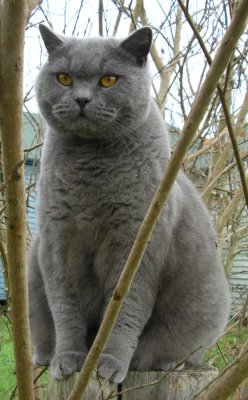
\includegraphics[width=2in]{images/cat.jpg}

\includegraphics[width=2in]{images/cat_tinted.jpg}
\end{figure}
\end{frame}
\subsection{MATLAB文件}

\begin{frame}
%The functions scipy.io.loadmat and scipy.io.savemat allow you to read and write MATLAB files. You can read about them in the documentation.

函数 \lstinline|scipy.io.loadmat| 和 \lstinline|scipy.io.savemat| 允许你读写 MATLAB 函数。具体请查看\href{http://docs.scipy.org/doc/scipy/reference/io.html}{文档}。
\end{frame}

\subsection{点之间的距离} %Distance between points
\begin{frame}
%SciPy defines some useful functions for computing distances between sets of points.

Scipy 定义了一些有用的函数,可计算集合中点之间的距离。

%The function scipy.spatial.distance.pdist computes the distance between all pairs of points in a given set:

函数 \lstinline|scipy.spatial.distance.pdist| 计算给定集合中所有两点之间的距离:
\lstinputlisting[]{code/scipy_pdist.py}

具体细节请阅读\href{http://docs.scipy.org/doc/scipy/reference/generated/scipy.spatial.distance.pdist.html}{文档}。
%A similar function (scipy.spatial.distance.cdist) computes the distance between all pairs across two sets of points; you can read about it in the documentation.

函数 \lstinline|scipy.spatial.distance.cdist| 可以计算不同集合中点的距离。
\end{frame}

\section{Matplotlib}

%Matplotlib is a plotting library. In this section give a brief introduction to the matplotlib.pyplot module, which provides a plotting system similar to that of MATLAB.

Matplotlib 是一个绘图库。这里简要介绍matplotlib.pyplot模块,功能和MATLAB的绘图功能类似。

\subsection{Plotting}

%The most important function in matplotlib is plot, which allows you to plot 2D data. Here is a simple example:

matplotlib中最重要的函数是 \lstinline|plot|,该函数允许你绘制 2D 图形。这是一个简单的例子:
\lstinputlisting[]{code/matplotlib_plot.py}

%Running this code produces the following plot:

运行该代码可生成下图:
\begin{figure}[htbp]
        \centering
        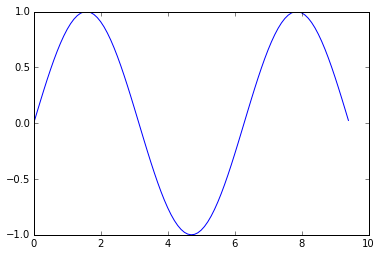
\includegraphics[width=3in]{images/sine.png}
\end{figure}



%With just a little bit of extra work we can easily plot multiple lines at once, and add a title, legend, and axis labels:

只需少量工作,就可以一次绘制多条曲线,并添加标题、图示和轴标:
\lstinputlisting[]{code/matplotlib_plot1.py}

\begin{figure}[htbp]
        \centering
        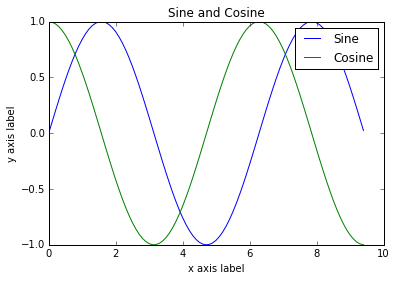
\includegraphics[width=3in]{images/sine_cosine.png}
\end{figure}


\subsection{Subplots}

%You can plot different things in the same figure using the subplot function. Here is an example:

可以使用 \lstinline|subplot| 函数来在一幅图中画不同的东西:  

\lstinputlisting[]{code/matplotlib_subplot.py}

\begin{figure}[htbp]
        \centering
        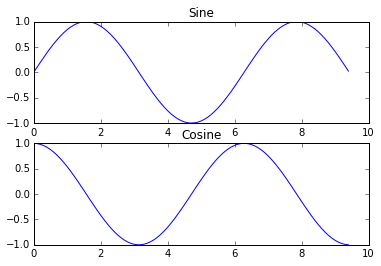
\includegraphics[width=3in]{images/sine_cosine_subplot.png}
\end{figure}


\subsection{Images}

%You can use the imshow function to show images. Here is an example:
你可以使用 \lstinline|imshow| 函数来显示图像。例如: 
\lstinputlisting[]{code/matplotlib_imshow.py}

\begin{figure}[htbp]
        \centering
        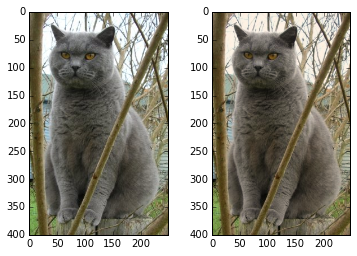
\includegraphics[width=4in]{images/cat_tinted_imshow.png}
\end{figure}

\end{document}
